% -*- TeX-master: "main"; fill-column: 72 -*-

\section{Proposed syntax and semantics}
\label{syntax}

In this section, we define the syntax and semantics of the COMBINE 
Archive. We expound on the various data types and constructs defined, 
then in \sect{examples}, we provide complete examples of archives. 

\subsection{The archive format}

The COMBINE archive is encoded using the "{O}pen 
{M}odeling {EX}change format" (OMEX). The archive itself is a "zip" file \cite{zipFile}. Zip is a file format used for data compression and archiving. A zip file contains one or more files that have been compressed, to reduce file size, or stored as is. The technical specification of the ZIP format is available from the PKWARE website \cite{zipSpec}.

\subsection{COMBINE archive extensions}
\label{combine-archive-extensions}
The extension for the COMBINE archive is \token{.omex}

Additional extensions are available to indicate what is the main standard format used within the archive. This help users to choose between different archives, and select appropriate software tools and in particular parsers. As such, the purpose of the extensions is different from the master attribute of the manifest file, described in section \ref{content-class}, which is read by the processing software once the archive is loaded and parsed. Currently, the following extensions are specified:

\begin{itemize}
	\item {\token{.sedx} - SED-ML archive} \citep{Waltemath:2011}
	\item {\token{.sbex} - SBML archive} \citep{hucka:2003}
	\item {\token{.cmex} - CellML archive} \citep{Cuellar:2003}
	\item {\token{.neux} - NeuroML archive} \citep{Gleeson:2010}
	\item {\token{.phex} - PharmML archive} \citep{Moodie:2013}
        \item {\token{.sbox} - SBOL archive} \citep{Galdzicki:2014}
\end{itemize}

Note that a COMBINE archive may contain files in several different standard formats. Therefore the specific extension is only an indication. For instance, a database of models could distribute archives of the same models, encoded encoded in SBML with the extension \token{.sbex} and encoded in CellML with the extension \token{.cmex}. However, archives containing models in both formats could also be distributed and the extension \token{.omex} used. If the archives contain SED-ML files, the extension \token{.sedx} could be used and the selection between the model formats be devolved to the SED-ML file. 

\subsection{Content of the archive}

The archive contains: 

\begin{enumerate}
	\item {
	
     a mandatory manifest file, called \token{manifest.xml}, always located at the 
     root of the archive, that describes the location and the type of each 
     data file contained in the archive plus an entry describing 
     the archive itself.
     
     The location of those files is defined by a relative path. In the current 
     version of the COMBINE archive, all the files described must be included 
     in the archive itself. It is envisioned that in the future the manifest 
     might list files located elsewhere, using valid and resolvable http 
     URIs. 

	}
	\item {
     metadata files containing clerical information about the 
     various files contained in the archive, and the archive itself. A best practice is to include only one file for each file format metadata called \token{metadata.*} (where \token{*} means the 
     suitable file extension)
	}
	\item {all the remaining files necessary to the model and simulation project. }

\end{enumerate}

\subsection{Namespace URI and other declarations necessary}
\label{xml-namespace}

In order to uniquely identify the manifest file and the whole archive, OMEX defines two namespaces.

The namespace URI for OMEX: 

\begin{quote}
\uri{http://identifiers.org/combine.specifications/omex}
\end{quote}

The namespace URI for the COMBINE archive manifest: 

\begin{quote}
\uri{http://identifiers.org/combine.specifications/omex-manifest}
\end{quote}

Versioned URIs will be generated as needed, following the practices of COMBINE standards.


\subsection{Primitive data types}
\label{primtypes}

The COMBINE archive uses the XML Schema 1.0 data types~\citep{biron:2000}.
More specifically we make use of \primtype{string} and \primtype{boolean}.

\subsection{The \token{manifest.xml} file and the \class{OmexManifest} class}
\label{manifest-class}

One file must be present at the root of any COMBINE archive, names \token{manifest.xml}. This file contains an instantiation of the \OmexManifest class. 

It contains a number of \Content children, one of which represents the COMBINE archive itself. 

A valid manifest needs to have at least one entry, declaring the archive itself, but may 
contain as many entries as needed. All the files present in the archive but one must be listed in the manifest. The only optional entry describes the manifest.xml file. Indeed the presence of manifext.xml is mandatory and its declaration is not necessary for parsing (since the software would have already parsed it to access the declaration!).

\begin{figure}[h!]
  \centering
  % Requires \usepackage{graphicx}
  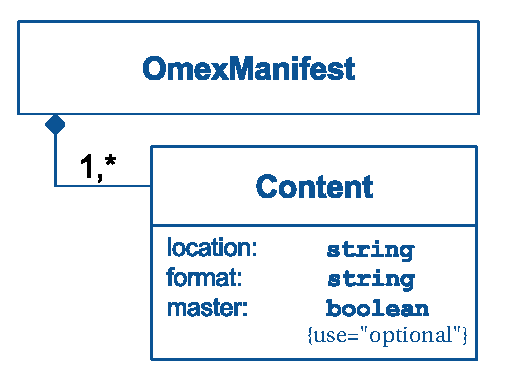
\includegraphics[width=6cm]{images/OmexManifest.pdf}\\
  \caption{A UML representation of the Manifest. Each manifest contains a number of Content elements.}
  \label{fig:combine_uml}
\end{figure}

\subsection{The \class{Content} class}
\label{content-class}
An entry in the \OmexManifest is represented by the \Content class. It declares a file in the \emph{COMBINE archive}. A content element possesses two required attributes, \token{location} and \token{format}, as well as an optional one, \token{master} 

\paragraph{The \token{location} attribute}
The \token{location} attribute of type 
\token{string} is required. It represents the relative location of an entry within the 
archive. The archive is represented by a dot \token{'.'}. 

\paragraph{The \token{format} attribute}
The \token{format} attribute of type \token{string is required}. It 
indicates the file type of the \Content element. The allowed values fall in two categories. Either the format 
denotes one of the COMBINE standards, in which case the \token{format} 
is the corresponding \token{Identifiers.org} URI. Or the 
\token{format} represents an Internet Media type \citep{rfc2046}, in which case the \token{format} 
indicates this media type.

Using an \token{Identifiers.org} URI allows to unambiguously define a COMBINE format, including the precise version used. For example, the identifier: \token{http://identifiers.org/combine.specifications/sbml} would denote that the file declared by the \Content 
element is encoded in the SBML format. That might be sufficient, as tools supporting one version of SBML often
support others as well. However, if the software creating the COMBINE archive wanted to be more precise, it could specify that the document is encoded in SBML Level 2: 

\begin{quote}
\token{http://identifiers.org/combine.specifications/sbml.level-2}
\end{quote}

or even:

\begin{quote}
\token{http://identifiers.org/combine.specifications/sbml.level-2.version-4}.
\end{quote}


The Internat Media type \token{purl.org} URI should be of the form \token{http://purl.org/NET/mediatypes/}
followed by the Media type name. Here are a few examples:

\begin{example}
    for png (Portable Network Graphics) http://purl.org/NET/mediatypes/image/png
    for pdf (Portable Document Format) http://purl.org/NET/mediatypes/application/pdf
    for sbml http://purl.org/NET/mediatypes/application/sbml+xml
\end{example}

If both an \token{Identifiers.org} URI and an internet MIME type are available for one given format, the
\token{Identifiers.org} URI must be used. Therefore the latter example should not be used. 

When creating a new COMBINE archive, the URI form should always be used for Media types. However, you may encounter some
old COMBINE archives that use directly the Media type name for the format attribute, not in the URI form.

\paragraph{The \token{master} attribute}
\label{active_document}
The \token{master} attribute of type \token{boolean} optional. When set to "true", it 
indicates that the file declared by the content element should be used first when 
processing the content of the archive. The file can be for instance the description of an upper model in a 
composed model, itself declaring the various submodels; a simulation description, 
declaring the different model descriptions and data sources used in the 
experiment. In most cases, one content element per archive will have its \token{master} 
attribute set to \token{true}.

For example the reading the snippet below, a software program should decide to present to the users first the file pointed by  \token{location="simulation.xml"}.

\begin{example}
<?xml version="1.0" encoding="utf-8"?>
<omexManifest xmlns="http://identifiers.org/combine.specifications/omex-manifest">
    <content location="." format="http://identifiers.org/combine.specifications/omex"/>
    <content location="model/model.xml" 
        format="http://identifiers.org/combine.specifications/sbml"/>
    <content location="simulation.xml" master="true"
        format="http://identifiers.org/combine.specifications/sed-ml"/>
</omexManifest>
\end{example}

To simplify the identification, by a user or software, of the formats used by the documents inside an archive, file extensions 
(see also \ref{combine-archive-extensions}) can also be used. For instance, the archive containing the manifest file shown in the example above, could have the extension \token{.sbex}, to indicate that the software reading the archive need
to support the \token{SBML} format to be able to interpret the content of the archive. If the software
does support SED-ML as well as SBML, it should load the SED-ML file as the creator of the archive indicated
it to be the '\token{master}' file. If the software does not support SED-ML, it can still open the SBML document, ignoring
the master attribute.

Alternatively, if a software does not support either SBML or SED-ML it can choose to disregard the \token{master} attribute and the archive extension to present to the user the files present in the archive that it supports such as a PDF document of a  diagram describing the model, 

In some cases, the \token{master} attribute is more precise than the information given by the archive file
extension.


\begin{example}
<?xml version="1.0" encoding="utf-8"?>
<omexManifest xmlns="http://identifiers.org/combine.specifications/omex-manifest">
    <content location="." 
        format="http://identifiers.org/combine.specifications/omex"/>
    <content location="main-model.xml" master="true"
        format="http://identifiers.org/combine.specifications/cellml.1.1"/>
    <content location="submodel1.xml" 
        format="http://identifiers.org/combine.specifications/cellml.1.1"/>
    <content location="submodel2.xml" 
        format="http://identifiers.org/combine.specifications/cellml.1.1"/>
</omexManifest>
\end{example}

In this case, the archive contains a modular CellML model. The file extension \token{cmex} is not sufficient to know which file should be processed first since there are several CellML files. The \token{master} attribute allows the software
to know it should process \token{main-model.xml} first.

Ideally, COMBINE archives should contain only one model and should have only one \token{master} attribute set to \token{true}. However, in some cases, the creator of the archive might want to set several \token{master} attribute to \token{true}, for instance to indicate alternative renditions of a model in different formats, or to bundle together several models described in the same publication. In that case the reading software are free to open a specific file, all the files tagges as master, or display a dialog box to the user offering a choice. This might create some confusion as opening the same archive several times in the same software might result in a different model loaded. One option would be to not set any \token{master} attribute to \token{true}, being aware that proper interpretation of the archive migh be difficult, in particular for modular models.  


\subsection{Advised format for the archive metadata}

Any type of file can be included in a COMBINE archive, and therefore any 
type of metadata format. However, in the interest of interoperability, 
and to ease the development of software support for metadata, a 
recommended format is provided as part of the specification of the 
archive. 

The recommended format is based on several standards developed by other 
organisations: 

\begin{itemize}
	\item  {
	
     The \href{http://www.w3.org/RDF/ }{ Resource Description Format} of the 
     W3C, in particular its terms:
     \begin{itemize}
		\item \token{RDF}, 
		\item \token{Description}.
	\end{itemize}
	}
	\item  {

	FIXME (vCard Ontology) vCard 4 (\cite{rfc6350}), a file format standard for electronic business 
    cards, in particular its terms:
    	\begin{itemize}
		\item \token{hasName}, 
		\item \token{family-name}, 
		\item \token{given-name}, 
		\item \token{hasEmail},
		\item \token{organization-name}.
	\end{itemize}

	More information on how to use vCard in RDF can be found 
    on the W3C website\footnote[1]{\url{http://www.w3.org/TR/vcard-rdf/ }}.
	
	}
	\item {
	
	Metadata terms\footnote[2]{\url{http://dublincore.org/documents/dcmi-terms/}} of 
	the Dublin Core Metadata Initiative, in particular the terms: 

	\begin{itemize}
		\item \token{description}, 
		\item \token{creator}, 
		\item \token{created}, 
		\item \token{modified},
		\item \token{W3CDTF}.
	\end{itemize}
		
	More information on the use of Dublin Core in RDF can be found 
	on the Dublin Core website{\footnote[3]{\url{http://dublincore.org/documents/dc-rdf/}}}. 
	
	More information is available about the definition of the date format used within \token{dcterms:created} and 
	\token{dcterms:modified} elements{\footnote[4]{\url{http://www.w3.org/TR/NOTE-datetime}}}.
	}
\item {The BioModels qualifiers FIXME
}
\end{itemize}

Users of the COMBINE standards may already be familiar with this 
approach, as it is also taken by SBML, SED-ML, SBGN-ML. 
Note however that the format here slightly differs from the controlled 
annotations of SBML. The differences have been made to address inconsistencies 
in the SBML vCard specification and to follow W3C recommendations {\footnote[4]{\url{http://www.w3.org/TR/vcard-rdf/}}} . The changes are: FIXME (URL)

\begin{itemize}
	\item  "n" becomes "hasName" 
	\item  "Family" becomes "family-name" 
	\item  "Given" becomes "given-name" 
	\item  "EMAIL" becomes "hasEmail" 
	\item  "Orgname" becomes "organization-name" 
\end{itemize}

A \textit{COMBINE archive} can include multiple metadata elements adding information about different content. To 
identify the file a metadata element refers too, the
\token{rdf:about} attribute should use the same value also used 
in the \token{location} attribute of the respective \Content element, e.g.

\begin{example}
<?xml version="1.0" encoding="UTF-8"?>
<rdf:RDF xmlns:rdf="http://www.w3.org/1999/02/22-rdf-syntax-ns#" 
         xmlns:dcterms="http://purl.org/dc/terms/" 
				 xmlns:vCard="http://www.w3.org/2006/vcard/ns#">
   <rdf:Description rdf:about="simulation.xml">
   ...
	 </rdf:Description>
</rdf:RDF>
\end{example}

A complete example of 
the metadata related to a simulation description contained in a COMBINE 
archive is described in \ref{examples}. 


